% Drawing 70/04-6 -- folder 70, batch 04, archive page 75 (PDF page 76).
% Transcription: Petit croquis en marge : le rectangle d'or de sommets $s_1$, $s_0$, $-s_0$, $-s_1$, côtés $x$ et $y$.
% Kind: golden rectangle. Method 2 (schematic redraw from the facsimile). Status: ok.
% Notes: Rectangle s_1, s_0 (top), -s_0, -s_1 (bottom), with the two axes crossing it; side labels x (on the axis) and y (top). Strokes drawn heavily.
% Coordinates: 1 unit = 1 mm = 1/100 of the crop width (bbox in page fractions: [0.04, 0.46, 0.2, 0.6]).
% Redrawn by Claude (claude-opus-5-5), issue #73, 2026-11-07; not checked by a human; not compiled (no TeX in the session).
% Rights: reproduces part of the work -- behind RENDER_TRANSCRIPTS, never published by itself.
\documentclass[tikz,border=3pt]{standalone}
\usepackage{amsmath,amssymb}
\usetikzlibrary{patterns,arrows.meta}
\tikzset{pencil/.style={black!45}, struck/.style={black!35}, mark/.style={circle,draw,inner sep=1.3pt}, pt/.style={circle,fill,inner sep=0.9pt}, opt/.style={circle,draw,fill=white,inner sep=1.1pt}}
\begin{document}
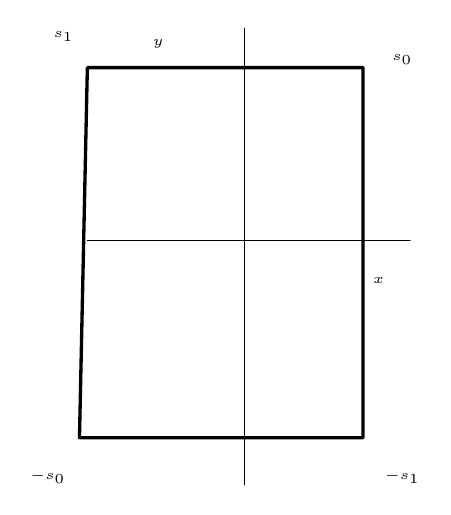
\begin{tikzpicture}[x=1mm,y=1mm,line cap=round,line join=round,font=\scriptsize]
\draw[very thick] (57,-25) -- (92,-25) -- (92,-72) -- (56,-72) -- cycle;
\draw (77,-20) -- (77,-78);
\draw (57,-47) -- (98,-47);
\node[inner sep=1pt] at (54,-21) {\tiny $s_1$};
\node[inner sep=1pt] at (97,-24) {\tiny $s_0$};
\node[inner sep=1pt] at (52,-77) {\tiny $-s_0$};
\node[inner sep=1pt] at (97,-77) {\tiny $-s_1$};
\node[inner sep=1pt] at (66,-22) {\tiny $y$};
\node[inner sep=1pt] at (94,-52) {\tiny $x$};
\end{tikzpicture}
\end{document}
